\chapter{Metodología}  \label{metodologia}

En este capítulo voy a describir los experimentos que voy a realizar en el estudio, las herramientas que usaré y cuales son mis hipótesis iniciales.

\section{Experimentos a realizar}

Para estudiar como afecta la cuantificación a los distintos algoritmos de entrenamiento presentados voy a realizar varios entrenamientos con distintos parámetros sacando métricas que me den información acerca de su desempeño y del comportamiento de sus pesos. 

Los parámetros que voy a modificar en cada uno de los entrenamientos son los siguientes:
\begin{itemize}
    \item \textbf{Profundidad de la red}: Cantidad de capas que conforman la red.
    \item \textbf{Anchura de las capas}: Número de neuronas en las capas ocultas.
    \item \textbf{Función de cuantificación}: Función usada en el proceso de cuantificación de los pesos.
    \item \textbf{Nivel de cuantificación}: Especifica si la cuantificación se realiza a nivel global, toda los pesos de la red estarán en un rango [min\_global, max\_global] fijado previamente antes de la ejecución; o local, los pesos de cada capa se cuantificarán en el rango [min(capa),max(capa)], este rango irá cambiando a lo largo del entrenamiento.
    \item \textbf{Número de bits}: Cantidad de bits que se usarán en el proceso de cuantificación.
\end{itemize}

Los parámetros de profundidad y anchura afectan a la arquitectura de la red mientras que la función de cuantificación, nivel de cuantificación y el número de bits modifican el proceso de cuantificación. 

\subsection{Arquitecturas}
Las arquitecturas analizadas han sido seleccionadas partiendo del estudio \cite{10481/72221}. Se ha seleccionado la arquitectura que mejor desempeño tenía por debajo de las 4096 sinapsis, número de sinapsis por chip, con la idea de evaluar una red que pueda ser ejecutada con la necesidad de un único crossbar array. Para estudiar como afecta profundidad y anchura se han seleccionado de manera arbitraria 5 arquitecturas extra para ver si estos parámetros permiten mejorar el desempeño de las redes cuantificadas. A continuación se muestran las arquitecturas seleccionadas:

\begin{table}[H]
    \renewcommand{\arraystretch}{1.5}
    \centering
    \begin{tabular}{ccc}
        \toprule[0.75mm]
        {\textbf{Capas Ocultas}} & \textbf{Unidades ocultas} & \textbf{Sinapsis} \\
        \hline
        1 & 4 & 3190\\
        \hline
        6 & 50 & 49960\\
        \hline
        1 & 100 & 79510\\
        \hline
        2 & 100 & 89610 \\
        \hline
        1 & 50 & 39760 \\
        \hline
        2 & 50 &  42310\\
        \bottomrule[0.75mm]
    \end{tabular}
    \caption{Arquitecturas FdNN}
    %\label{tab:my_label}
\end{table}

Todos estos modelos siguen el esquema fully connected neural network (redes totalmente conectadas), es decir, todas las neuronas están conectadas con todas las neuronas de la capa previa y de la capa posterior.


\begin{figure}[H]
\centering
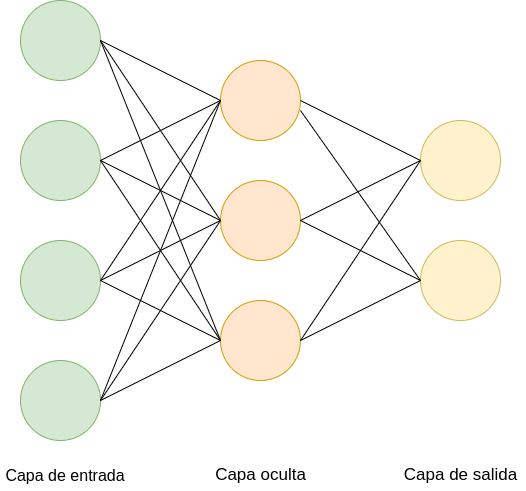
\includegraphics[width=0.5\textwidth]{imagenes/fdnn.drawio.png} 
\caption{Red totalmente conectada}
\end{figure}

\subsection{Bases de datos}

Las bases de datos que han sido seleccionadas para realizar el benchmark son MNIST \cite{7966217} y Fashion-MNIST \cite{DBLP:journals/corr/abs-1708-07747}. Ambas bases de datos son usadas para evaluar el rendimiento de algoritmos de aprendizaje automático. A día de hoy ya se han conseguido resolver casi a la perfección pero aun así se siguen usando para evaluar modelos que se encuentran en sus primeras fases de estudio, como es nuestro caso con los modelos cuantificados.  

MNIST es una base de datos de números escritos a mano, estos números se representan por imágenes de 28x28 en escala de grises, contando con un total de 70000 imágenes etiquetadas entre 0-9. Se dividen en un cojunto de entrenamiento de 60000 imágenes y un conjunto de test de 10000 imágenes.

\begin{figure}[H]
    \centering
    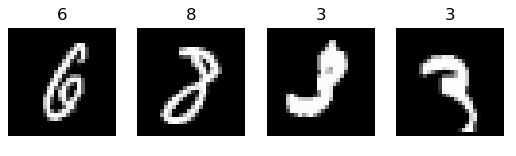
\includegraphics[width=1\textwidth]{imagenes/mnist.png}
    \caption{MNIST}
\end{figure}

Fashion MNIST es una base de datos de prendas de ropa (Camisetas/tops, pantalones, suéteres, vestidos, abrigos, sandalias, camisas, zapatillas, bolsos y botas) con las mismas características que MNIST, un total de 70000 imágenes en escala de grises de 28x28, 60000 destinadas a entrenamiento y 10000 destinadas a test. A pesar de tener un mismo tamaño se trata de una base de datos más compleja de aprender y que representa mejor los problemas reales.

\begin{figure}[H]
    \centering
    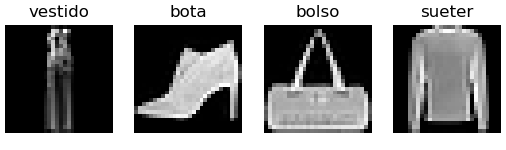
\includegraphics[width=1\textwidth]{imagenes/fmnist.png}
    \caption{FMNIST}
\end{figure}

Al tener ambas las mismas características no hace falta que modifiquemos las estructuras de las redes, pues la entrada, imágenes de 28x28, y la salida, clasificación entre 10 clases, son las mismas.

\subsection{Método de cuantificación}

Ya tenemos las redes que vamos a usar en la experimentación y sobre que conjunto de datos las vamos a ejecutar. Ahora toca explicar como voy a simular de manera aproximada el comportamiento de las redes neuronales en circuitos neuromórficos. Como se ha mencionado en los preliminares \ref{preliminares} los memristores cuentan con una precisión numérica limitada de 1 a 3 bits. Por lo tanto, los pesos se tienen que codificar con en esta precisión numérica. Las funciones de activación, las entradas y las salidas no es necesaria cuantificarlas debido al carácter analógico de los circuitos neuromórficos. Teniendo esto en cuenta, habrá que modificar el proceso de entrenamiento para que cada vez que se actualicen los pesos, cuantificarlos dentro de los rango definidos. Según hemos establecido los parámetros, se pueden diferenciar dos tipos de cuantificación, una a nivel global, mismo rango para toda la red, y nivel local, un rango distinto por cada capa. El nivel global es bastante simple, se define un rango inicial que tendrá x valores posibles (en función del número de bits) y los pesos solo podrán tomar esos valores. Es la simulación más fiel a la realidad debido a que los memristores se suelen fabricar con los mismos niveles (rango de valores). Mientras tanto, la cuantificación local consiste en cada vez que se actualice la red, se cuantifica capa por capa, cogiendo los máximos y mínimos de cada capa y cuantificando entre esos dos valores. Esto provoca que el intervalo sea dinámico durante la ejecución, cosa que no ocurre en la realidad. Esta cuantificación se ha explorado con la idea de estudiar que ocurriría si cada capa tuviera un rango de valores distintos, y si implica una mejora notable como para estudiar en un futuro si tener rangos distintos por capas es rentable, y de ser así, estudiar como seleccionar dichos rangos.  

La cuantificación también se verá afectada por la función que usemos para cuantificar ASYMM \ref{asymm} o SYMM \ref{asymm}, en el caso de la función ASYMM el rango estará comprendido entre el máximo y mínimo de la capa, mientras que con la función SYMM el intervalo es simétrico con respecto al 0 cuyos extremos son [-maximo absoluto, maximo absoluto].

\subsection{Métricas y función de error}

Definida la fase experimental ahora queda describir cómo se van a evaluar los resultados. Para ello tendremos que elegir bien las métricas que usaremos para valorar el desempeño de las redes entrenadas y cuál será la función de error que usaremos para ajustar los modelos.

Ambas bases de datos se engloban dentro de los problemas de clasificación, es decir, dado una muestra tendremos que establecer a qué métrica pertenece. Por lo tanto, métricas y función de error tienen que pertenecer a la clase de los problemas de clasificación. 

\subsubsection{Función de error}

Para seleccionar la función de error tenemos que tener en cuenta el tipo de problema y la función de salida de nuestra red. Al estar ante un problema de clasificación la salida será un vector de n resultados que indique la probabilidad que tiene la entrada de pertenecer a cada una de las clases, siendo n el número de clases. Las funciones de salida que se usan en estos problemas son la función sigmoid y softmax. La función sigmoid hace que cada uno de los elementos del vector de salida tenga un valor entre 0 y 1, el cual indicará el grado de pertenencia a cada una de las clases. Para clasificar una entrada se le asignará la etiqueta de la clase que sobrepase un umbral, como puede ser 0.75. Esto provoca que para una entrada pueda haber varias etiquetas, por lo tanto esta función no es útil para nuestro problema. Por su parte, la función softmax hace que los valores del vector de salida estén entre 0 y 1 y la suma total sea 1. De esta forma por cada entrada solo se asignará una clase, la que mayor probabilidad tenga. Los problemas seleccionado tienen clases disjuntas por lo que la función que tendremos que usar es la función softmax.  

Partiendo de nuestra función de salida tendremos que elegir como calcular el error de nuestra red. Sabemos que estamos en un problema de clasificación por lo que la forma en la que tenemos que ajustar nuestro modelo es mediante la máxima verosimilitud. La máxima verosimilitud es un método para ajustar los parámetros de un modelo para que pueda hacer predicciones cuya distribución de probabilidad coincida con la distribución de probabilidad de las etiquetas. Consiste en un problema de optimización en el que se intenta hacer mínima la diferencia entre ambas distribuciones de probabilidad. Para calcular esta diferencia se usa la función de error de la entropía cruzada. Por lo tanto, en el framework que vamos a usar, que es PyTorch (en el siguiente apartado se aclara su elección) tendremos que encontrar la función que calcule la entropía cruzada. Existen dos alternativas: corss entropy loss y negative log likelihood. Ambas calculan la entropía cruzada pero se diferencian en el tipo de entrada que aceptan. La cross entropy loss espera que nuestra red ofrezca los resultados sin transformación, es decir, que la salida no sean probabilidades. Por su parte la negative log likelihood si que espera que la salida de nuestra red sean probabilidades. Como nuestra red usa la función softmax, las salidas están codificadas como probabilidades, la función negative log likelihood será la función de error que tendremos que usar.

\subsubsection{Métricas}

Una vez entrenado el modelo se deberá de evaluar que tan bueno es. Para ello se hará uso del conjunto de test, el cual no se ha usado durante ningún momento del entrenamiento. 

Un clasificador es más bueno que otro si es capaz de ajustar mejor la distribución de probabilidad de la muestra. Pero, ¿cómo podemos medir este ajuste?. Una aproximación es: dado un conjunto de test, medir que porcentaje del total ha conseguido clasificar correctamente, es decir, la precisión de nuestro modelo. Cuanto más muestras clasifique correctamente, mejor será nuestro modelo. Pero esto no siempre es así. En el caso de problemas cuyas clases no estén equilibradas, es decir, que no haya el mismo número de muestras de cada clase, podemos equivocarnos al tomar esta medida, pues se tendrá que tener en cuenta esta descompensación. Ejemplo de ello son los problemas de predicción de cáncer de mama. La mayoría de las muestras son muestras negativas, y la minoría positivas, por lo que si un modelo solo predijese valores negativos tendría una precisión muy alta si lo medimos erróneamente. En los dos problemas que hemos seleccionado todas las clases están equilibradas por lo que no tenemos que preocuparnos por compensar el desequilibrio en el cálculo de la métrica. Por lo tanto, la métrica que usaremos será el accuracy (precisión).

\begin{equation}
    precision = \frac{Muestras\ clasificadas\ correctamente}{Total\ de\ muestras}x100
\end{equation}

\section{Herramientas}

A continuación, voy especificar cuales son las herramientas que voy a emplear durante la práctica.  

El lenguaje que he seleccionado para la implementación de este estudio es python. Este lenguaje es uno de los más usados a nivel global, y el más usado en el ámbito del machine learning \footnote{\url{https://www.kaggle.com/kaggle-survey-2021}}. El motivo de su amplia utilización en machine learning es debido a su fácil depuración, vital en este campo de desarrollo, y a la gran cantidad de frameworks que facilitan las tareas de desarrollo, implementación y despliegue. Entre los frameworks más famosos y que se centran en el desarrollo de redes neuronales nos encontramos TensorFlow \footnote{\url{https://www.tensorflow.org/}} y PyTorch \footnote{\url{https://pytorch.org/}}. Tensorflow fue desarrollado desde un inicio para tareas de visión por computador, permitiendo programar modelos de redes neuronales con pocas lineas de código. Tiene un gran rendimiento y un gran conjunto de herramientas de desarrollo, sin embargo, tiene el inconveniente de que para tareas tan importantes como el debugging es necesario el uso de herramientas específicas, tfdbg. Por su parte, PyTorch también es un framework muy eficiente, pero es más fácil de debuggear (no se necesita aprender ninguna herramienta específica) debido a que hace uso de lo que se conoce como grafo computacional dinámico, mientras que TensorFlow usa una aproximación estática \cite{9049650}. Además, PyTorch es el framework que más se suele utilizar en investigación, ejemplo de ello es que todos los papers que he seleccionado que estudian alternativas del backpropagation realizan su implementación en PyTorch.  En conclusión, por su accesibilidad y por la disponibilidad de los algoritmos que voy a estudiar, el framework que he seleccionado para realizar mi proyecto es PyTorch.


Además de un framework de desarrollo de redes neuronales tendré que seleccionar las bibliotecas necesarias para obtener gráficos, realizar cálculos matriciales e implementar los algoritmos que he seleccionado. Con respecto a las gráficas, la biblioteca más utilizada es matplotlib \footnote{\url{https://matplotlib.org/}}. Tiene una gran cantidad de herramientas para crear gráficos entendibles y de manera sencilla, lo que facilitará la presentación de los resultados. Para el manejo de vectores y matrices usaré la famosa biblioteca numpy \footnote{\url{https://numpy.org/}}, debido a su gran eficiencia y facilidad de uso. Finalmente, para la implementación de los algoritmos que han sido seleccionados para el estudio se usará los repositorios de github que se especifican en los respectivos papers. En el caso del FeedBack Alignment he usado el sitio web PapersWithCode \footnote{\href{https://paperswithcode.com/}{PapersWithCode}} para encontrar un repositorio donde se implementara dicho algoritmo. Como he mencionado en el párrafo anterior, todas las implementaciones han sido realizadas en PyTorch por lo que no habrá problemas de incompatibilidad. Los repositorios de los algoritmos son los siguientes: HSIC \footnote{\href{https://github.com/choasma/HSIC-Bottleneck}{HSIC}}, Synthetic Gradients \footnote{\href{https://github.com/koz4k/dni-pytorch}{Synthetic Gradients}} y FeedBack Alignment \footnote{\href{https://github.com/jsalbert/biotorch}{FeedBack Alignment}}.

\section{Hipótesis iniciales}

En este apartado voy a establecer unas hipótesis iniciales acerca de qué espero de la experimentación. Para ello partiré de los conocimientos adquiridos durante el estudio de los algoritmos seleccionados y de los métodos de cuantificación que voy a usar. 

Lo primero que se hará es ver los resultados que tiene cada uno de los modelos entrenados con los distintos algoritmos de entrenamiento sin ningún tipo de cuantificación. Según los resultados que ofrecen los papers todos deberían de llegar a resultados parecidos a los del backpropagation. Sin embargo, en los estudios se presentan arquitecturas grandes, en especial en el synthetic gradient que se usan para modelos muy profundos, por lo que en las arquitectura más pequeñas su comportamiento será más impredecible. Tras obtener los modelos sin cuantificar, se aplicaran las cuantificaciones y se observará como afecta la misma al entrenamiento. Según explican en el estudio de donde se han sacado las funciones de cuantificación, los modelos se pueden comprimir satisfactoriamente hasta los 6 bits, pasada esta barrera (2-3-4-5) los modelos pierden rendimiento de manera considerable. Teniendo en cuenta que estas cuantificaciones se realizaron sobre modelos ya entrenados, aplicar la cuantificación durante el entrenamiento puede llegar a producir peores resultados ya que durante el proceso de entrenamiento se pierde información por la cuantificación. Por lo tanto la barrera a partir de la cual las cuantificaciones no sean rentables aplicarlas tendrá que estar en torno a los 6 o 7 bits.  

De los algoritmos seleccionados el que mejor puede resistir la cuantificación es el HSIC, pues este algoritmo va calculando el gradiente capa por capa, sin propagación del error, por lo tanto, a menor cantidad de operaciones encadenadas, menor será la imprecisión numérica que introduce la cuantificación. Con respecto a las arquitecturas, pienso que estructuras más grandes pueden compensar la pérdida de precisión de las sinapsis, siendo la anchura de las capas el factor diferencial. En algoritmos como el backprop no interesa tener redes muy profundas debido al arrastre del error, por lo que será preferible tener arquitecturas menos profundas pero más anchas. 